\setchapterpreamble[u]{\margintoc}
\chapter{Case Studies}


\section{Introduction}

This chapter is a dissection of every important model I could think of. If our goal is to understand and critique AI models, then we need to understand the models themselves. I know of no better way to understand than to take models apart then rebuild them. In the first three chapters you learned all of the key topics you need to do a high-level dissection (if you haven't read the first three chapters please go back and do that). 

To facilitate this dissection I am going to use a tool called a \textbf{model card}. Model cards are a way to document the capabilities and limitations of your AI model. They are a useful tool for understanding your model, and for communicating its capabilities and limitations to others. Google (see \url{https://modelcards.withgoogle.com/face-detection}), Huggingface and even small makers of AI models produce model cards to help educate their users and developers, and as you can imagine no one reads them. 

In this chapter I am going to create and add commentary to model cards for many popular models. Whether you are a technial person or not I want you to be able to read and understand these, and eventually I want my notes or criticisms to become self-evident. My idea is that once you understand the data that is used to train a model and the domain that it is deployed, you can forecast its strengths and weaknesses almost automatically, let's try a few and see how it goes.

Note that I'll introduce these models in a very particular order. I'll also save the hairiest models (full-self driving and Skynet) their own chapters for a deeper discussion. Try and follow along in the order that I lay out here, but only until you get bored. Once you are bored and can forecast my criticisisms, you can skip around with impunity.

I'm happy to add future dissections or model cards to this chapter, so if you have a favorite model that you'd like to see dissection of, please let me know by emailing \href{mailto:brad@bradflaugher.com}{brad@bradflaugher.com}.

TODO Explain cost, quality and IP protection scores.

\subsection{Sucker Traps to Note When Analyzing Models}

\textit{"The sucker's trap is when you focus on what you know and what others don't know, rather than the reverse." Nassim Taleb, 2016}\cite{procrustes}

In chapters 1-3 there were a number of key concepts that we discussed that I'll call "Sucker Traps". Below is a list of those concepts that I will refer to regularly when discussing the model cards in this chapter:

\begin{itemize}
    \item \hyperref[sec:creative]{Creative or Critical}: The difference between a model that is used to inform a decision and a model that is used to make a decision.
    \item \hyperref[sec:explain]{Explainability}: The ability to understand why a model makes a particular prediction.
    \item \hyperref[sec:plag]{Plagiarism}: The capacity for a model to output copyrighted material from its training data.
    \item \hyperref[sec:drift]{Concept Drift}: The possibility and frequency of changes in the relationships in the training data.
    \item \hyperref[sec:janitor]{Editorializing}: The possibility of a modeler either explicitly or accidentally creating a biased training set and thus permanently shifting the outputs of the model away from reality.
\end{itemize}

\subsection{Key Terms}

\begin{itemize}
    \item \textbf{Accuracy:} The proportion of correctly classified examples to the total number of examples.
    \item \textbf{AUC:} Area under the Receiver Operating Characteristic (ROC) curve.
    \item \textbf{F1:} Harmonic mean of precision and recall.
    \item \textbf{False Negative (FN):} An instance that is actually positive but predicted as negative.
    \item \textbf{False Positive (FP):} An instance that is actually negative but predicted as positive.
    \item \textbf{Precision:} The proportion of correctly classified positive examples to the total number of positive examples predicted by the model.
    \item \textbf{Recall:} The proportion of correctly classified positive examples to the total number of actual positive examples.
    \item \textbf{True Negative (TN):} An instance that is actually negative and predicted as negative.
    \item \textbf{True Positive (TP):} An instance that is actually positive and predicted as positive.
\end{itemize}

\section{Model Cards}

\subsection{Fluid Dynamics}

\begin{itemize}
    \item \textbf{Description:} This model is intended to predict fluid flow patterns in various applications, such as aerodynamics, hydrodynamics, and weather forecasting.
    \item \textbf{Training Data:} The model is trained on a large dataset of numerical simulations of fluid flow patterns, which includes various geometries, fluid properties, and boundary conditions. The data is generated using well-established simulation tools such as the finite element method, finite volume method, or lattice Boltzmann method.
    \item \textbf{Evaluation:} The model is evaluated on a separate dataset of numerical simulations of fluid flow patterns that are not seen during training. The evaluation dataset includes a variety of geometries, fluid properties, and boundary conditions. The model's performance is measured using common metrics in fluid dynamics such as root-mean-square error (RMSE), mean absolute error (MAE), and correlation coefficient (R).
    \item \textbf{Limits and Risks:} This model is intended for scientific and engineering applications and is not directly used for decision-making that affects human lives. However, the model's predictions may indirectly affect human lives by informing engineering design or emergency response planning. It is important to validate the model's accuracy and uncertainty, and to communicate the limitations and assumptions of the model to stakeholders. The model assumes that the fluid flow is governed by the Navier-Stokes equations, which may not be accurate for highly turbulent or rarefied flows. The model may also be limited by the numerical precision and stability of the simulation tools used to generate the training data.
    \item \textbf{Common Myths or Misunderstandings:} Models of physical processes are excellent ways to experiment with the world as it is understood. However, if this model is trained on data that is not representative, it will lead its users to draw incorrect conclusions about the fluids that are being studied. This tool also should not be used by itself, think of this tool like the wind tunnels used to test the aerodynamics of a car. You probably want to road test the car as well, but if you can use a model to decrease the cost of your experimentation (by disqualifying models before tthey get to the road-test phase) then please do it. Said differently, don't let this model make any \hyperref[sec:creative]{critical decisions, but let it participate in the creative process}.

\textbf{Scores: Cost, Quality and IP Protection (setup format)}

\end{itemize}

\begin{marginfigure}[-5.5cm]
        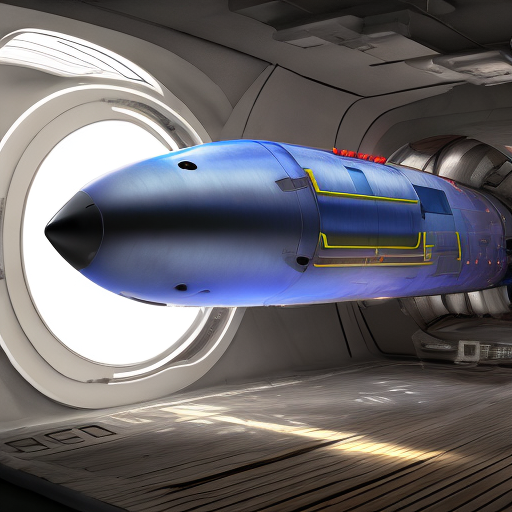
\includegraphics{fluid}
        \caption{"mdjrny-v4 a futuristic submarine in a wind tunnel" made with Mann-E}
        \labfig{fluid}
\end{marginfigure}

\subsection{Shakespearean Text} 

\begin{itemize}
\item \textbf{Description:} The Shakespearean Text Generator is a type of language model that's specifically designed to generate text in the style of William Shakespeare. It's based on deep learning algorithms, such as the Transformer architecture, and is trained on a large corpus of Shakespearean text. The model uses this training data to learn patterns and structures in Shakespeare's writing, and can then generate new text that mimics the style and language of the Bard himself.
\item \textbf{Training Data:} The Shakespearean Text Generator is trained on a large corpus of text written by William Shakespeare. This can include plays, sonnets, and other works by the Bard. The quality and quantity of the training data will impact the performance of the model, so it's important to use a high-quality corpus that accurately represents Shakespeare's writing.
\item \textbf{Evaluation:} The performance of the Shakespearean Text Generator can be evaluated using a variety of metrics, such as perplexity, BLEU score, or human evaluation. Human evaluation is particularly useful for language models like this one, as it allows experts in Shakespearean literature to assess the quality of the generated text and compare it to the real works of Shakespeare.
\item \textbf{Use Cases:}The Shakespearean Text Generator has a number of potential use cases, including:
    \begin{enumerate}
        \item Generating new Shakespearean-style plays or sonnets
        \item Analyzing Shakespeare's writing style and language
        \item Creating educational materials and games that teach students about Shakespeare and his works
        \item Providing inspiration for creative writing and poetry
        \end{enumerate}
\item \textbf{Limits and Risks:} Like any language model, the Shakespearean Text Generator has limitations and risks. One of the main limitations is that it may not always generate text that is grammatically correct or semantically meaningful. Additionally, the model may struggle to capture all of the nuances and complexities of Shakespeare's writing, and may generate text that is not true to the style or spirit of the Bard.
\item \textbf{Common Myths or Misunderstandings:}
There are a few common myths or misunderstandings about the Shakespearean Text Generator. One myth is that the model can perfectly recreate Shakespeare's writing, when in reality it can only generate text that is similar in style. It's a great \hyperref[sec:creative]{creative tool} but that's about it. You'll also of course run into issues of \hyperref[sec:plag]{plagiarism} and model outputs should be checked to see their similarity to Shakespeaere's actual work, compared to the whole internet, Shakespeare's corpus is very small and the model may have a tendency to output its training data in raw form.
\end{itemize}

\begin{marginfigure}[-5.5cm]
        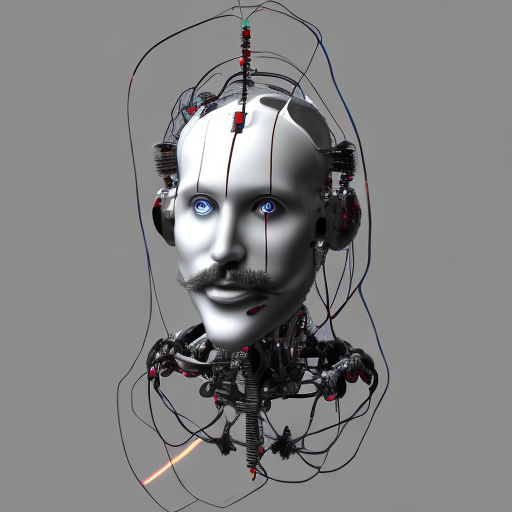
\includegraphics{shakebot}
        \caption{"mdjrny-v4 a robot that looks like shakespeare, with a few wires showing" made with Mann-E}
        \labfig{shakebot}
\end{marginfigure}

\subsection{Lithium Mining}

\begin{itemize} 
    \item \textbf{Description:} The Lithium Mining Site Classifier is a type of machine learning model that's designed to identify potential lithium mining sites based on a set of features. The model can be trained on a dataset of known lithium mining sites and their associated features, such as geology, topography, and geochemical data. The trained model can then be used to identify new potential mining sites by predicting the likelihood of a site containing lithium based on its feature set.
    \item \textbf{Training Data:} The Lithium Mining Site Classifier is trained on a dataset of known lithium mining sites and their associated features. This dataset should include a representative sample of mining sites, with a balanced distribution of positive (lithium-containing) and negative (non-lithium-containing) examples. The quality and quantity of the training data will impact the performance of the model, so it's important to use high-quality data that accurately represents the characteristics of lithium mining sites.
    \item \textbf{Evaluation:} The performance of the Lithium Mining Site Classifier can be evaluated using a variety of metrics, such as accuracy, precision, recall, and F1 score. These metrics can be used to compare different models and to track the progress of a model as it's trained on more data. Additionally, the model can be validated using independent test data that was not used during training, to assess its ability to generalize to new, unseen data.
    \item \textbf{Use Cases:} The Lithium Mining Site Classifier has a number of potential use cases, including:
    \begin{enumerate}
        \item Identifying new potential lithium mining sites
        \item Prioritizing exploration efforts by ranking the likelihood of a site containing lithium
        \item Supporting decision-making in the lithium mining industry by providing a quantitative assessment of the potential of a site
    \end{enumerate}
\item \textbf{Limits and Risks:} Like any machine learning model, the Lithium Mining Site Classifier has limitations and risks. One of the main limitations is that it may not always be accurate, and may misclassify sites as either positive (lithium-containing) or negative (non-lithium-containing). Additionally, the model may be biased towards certain features if the training data is not representative of the true distribution of mining sites.
\item \textbf{Common Myths or Misunderstandings:} There are a few common myths or misunderstandings about the Lithium Mining Site Classifier. One myth is that the model can always accurately identify lithium mining sites, when in reality it can only provide a prediction based on the information it was trained on. Another myth is that the model can replace the expertise of geologists and mining engineers, when in reality it is intended to support and enhance their decision-making processes. Don't expect this model to be able to \hyperref[sec:explain]{explain itself though}.
\end{itemize}

\begin{marginfigure}[-5.5cm]
        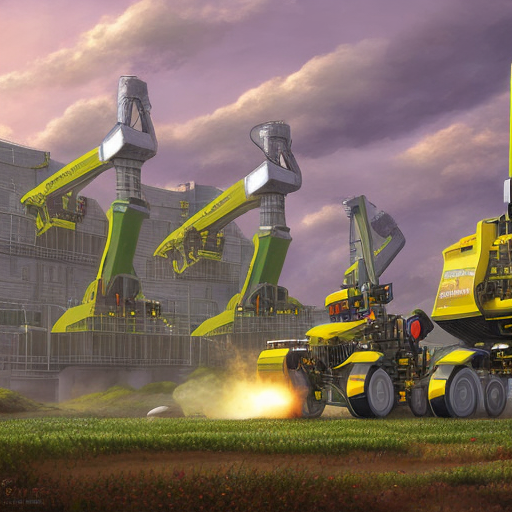
\includegraphics{lithium}
        \caption{"mdjrny-v4 a lithium mine, being mined by large robots made by John Deere" made with Mann-E}
        \labfig{lithium}
\end{marginfigure}

\subsection{Chess}

\begin{itemize}
    \item \textbf{Description:} The Chess Playing Model is a type of machine learning model that's designed to play the game of chess. It can be trained on a dataset of chess games and moves, and can then be used to make predictions about the best move to play in a given chess position. The model can be based on a variety of machine learning algorithms, including reinforcement learning, deep learning, or Monte Carlo tree search.
    \item \textbf{Training Data:} The Chess Playing Model is typically trained on a large dataset of chess games and moves, which can include both human and computer-generated games. The size and quality of the training data will impact the performance of the model, so it's important to use a diverse and representative dataset that accurately represents the game of chess.
    \item \textbf{Evaluation:} The performance of the Chess Playing Model can be evaluated using a variety of metrics, such as win rate, ELO rating, or human evaluation. These metrics can be used to compare different models and to track the progress of a model as it's trained on more data. Additionally, the model can be tested against human opponents or other chess-playing models to assess its ability to play the game effectively.
    \item \textbf{Use Cases:} The Chess Playing Model has a number of potential use cases, including:
        \begin{enumerate}  
            \item Playing the game of chess against human or computer opponents
            \item Analyzing chess games and moves to identify patterns and strategies
            \item Supporting chess education and training by providing a challenging opponent for students and players
            \item Developing new and innovative chess-related products and services
        \end{enumerate}
    \item \textbf{Limits and Risks:} Like any machine learning model, the Chess Playing Model has limitations and risks. One of the main limitations is that it may not always make the best move, and may make mistakes or suboptimal moves. Additionally, the model may be biased towards certain openings, strategies, or styles of play if the training data is not representative of the game of chess as a whole.
    \item \textbf{Common Myths or Misunderstandings:} There are a few common myths or misunderstandings about the Chess Playing Model. One myth is that the model can always beat human opponents, when in reality it can only make predictions based on the information it was trained on. Another myth is that the model can replace human expertise and creativity in the game of chess, when in reality it is intended to support and enhance human players' abilities. 
\end{itemize}

\begin{marginfigure}[-5.5cm]
        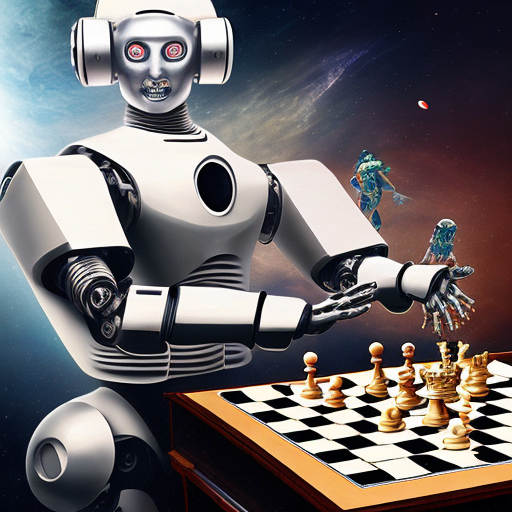
\includegraphics{chessmodelcard}
        \caption{"mdjrny-v4 human with a robot exoskeleton playing chess on a chessboard floating in space" made with Mann-E}
        \labfig{chessmodelcard}
\end{marginfigure}

\subsection{Go}

\begin{itemize}
    \item \textbf{Description:} The Go Playing Model is a type of machine learning model that's designed to play the game of Go. It can be trained on a dataset of Go games and moves, and can then be used to make predictions about the best move to play in a given Go position. The model can be based on a variety of machine learning algorithms, including reinforcement learning, deep learning, or Monte Carlo tree search.
    \item \textbf{Training Data:} The Go Playing Model is typically trained on a large dataset of Go games and moves, which can include both human and computer-generated games. The size and quality of the training data will impact the performance of the model, so it's important to use a diverse and representative dataset that accurately represents the game of Go.
    \item \textbf{Evaluation:} The performance of the Go Playing Model can be evaluated using a variety of metrics, such as win rate, ELO rating, or human evaluation. These metrics can be used to compare different models and to track the progress of a model as it's trained on more data. Additionally, the model can be tested against human opponents or other Go-playing models to assess its ability to play the game effectively.
    \item \textbf{Use Cases:} The Go Playing Model has a number of potential use cases, including:
        \begin{enumerate}  
            \item Playing the game of Go against human or computer opponents
            \item Analyzing Go games and moves to identify patterns and strategies
            \item Supporting Go education and training by providing a challenging opponent for students and players
            \item Developing new and innovative Go-related products and services
        \end{enumerate}
    \item \textbf{Limits and Risks:} Like any machine learning model, the Go Playing Model has limitations and risks. One of the main limitations is that it may not always make the best move, and may make mistakes or suboptimal moves. Additionally, the model may be biased towards certain openings, strategies, or styles of play if the training data is not representative of the game of Go as a whole.
    \item \textbf{Common Myths or Misunderstandings:} There are a few common myths or misunderstandings about the Go Playing Model. One myth is that the model can always beat human opponents, when in reality it can only make predictions based on the information it was trained on. If the game is played differently than the data it was trained on, the model is likely to fail. \textbf{This has happened in the past with seemingly "stupid" openings breaking world-class go playing models, it clearly illustrates the fragility of deep learning models in general, and their near total dependence on their training sets, as well as their lack of "knowledge" and "understanding" as commonly depicted\sidecite{sillygo}.} Another myth is that the model can replace human expertise and creativity in the game of Go, when in reality it is intended to support and enhance human players' abilities. Know and understand a the models \hyperref[sec:limits]{limitations} before you use it.
\end{itemize}

\begin{marginfigure}[-5.5cm]
        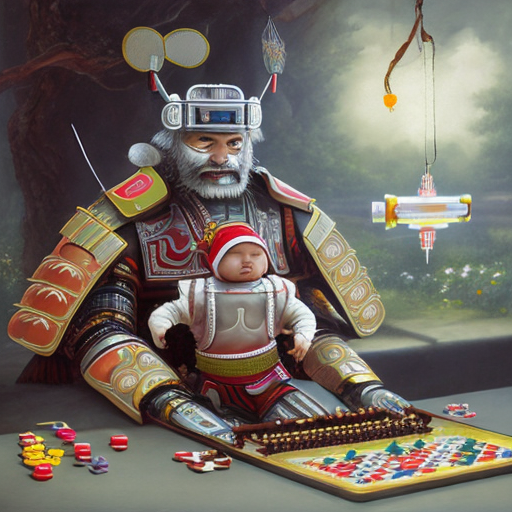
\includegraphics{gobaby}
        \caption{"mdjrny-v4 a robot samurai being frustrated by a baby playing go and winning" made with Mann-E}
        \labfig{gobaby}
\end{marginfigure}


\subsection{Large Stock Order}

\begin{itemize}
    \item \textbf{Description:} The Large NYSE Stock Order Classifier is a type of machine learning model that's designed to classify large stock orders on the New York Stock Exchange (NYSE) as either "aggressive" or "passive". Aggressive orders are those that are intended to have a significant impact on the stock price, while passive orders are those that are intended to have a minimal impact. The model can be trained on a dataset of large stock orders and their associated features, such as order size, order type, and trading volume.
    \item \textbf{Training Data:} The Large NYSE Stock Order Classifier is trained on a dataset of large stock orders and their associated features. This dataset should include a representative sample of aggressive and passive orders, with a balanced distribution of both types of orders. The quality and quantity of the training data will impact the performance of the model, so it's important to use high-quality data that accurately represents the characteristics of large NYSE stock orders.
    \item \textbf{Evaluation:} The performance of the Large NYSE Stock Order Classifier can be evaluated using a variety of metrics, such as accuracy, precision, recall, and F1 score. These metrics can be used to compare different models and to track the progress of a model as it's trained on more data. Additionally, the model can be validated using independent test data that was not used during training, to assess its ability to generalize to new, unseen data.
    \item \textbf{Use Cases:} The Large NYSE Stock Order Classifier has a number of potential use cases, including:
        \begin{enumerate}  
            \item Identifying aggressive and passive large stock orders on the NYSE
            \item Supporting market surveillance and regulatory compliance by detecting potential market manipulation
            \item Providing insights into market behavior and trends by analyzing the characteristics of aggressive and passive large stock orders
            \item Supporting algorithmic trading by classifying large stock orders in real-time
        \end{enumerate}
    \item \textbf{Limits and Risks:} Like any machine learning model, the Large NYSE Stock Order Classifier has limitations and risks. One of the main limitations is that it may not always be accurate, and may misclassify orders as either aggressive or passive. Additionally, the model may be biased towards certain features if the training data is not representative of the true distribution of large NYSE stock orders.
    \item \textbf{Common Myths or Misunderstandings:} There are a few common myths or misunderstandings about the Large NYSE Stock Order Classifier. One myth is that the model can always accurately classify aggressive and passive orders, when in reality it can only provide a prediction based on the information it was trained on. Another myth is that the model can replace human expertise and judgement in market surveillance and regulatory compliance, when in reality it is intended to support and enhance human decision-making processes. This might be a great performing model for a time, but consider that the players in the market change quite often, and you while you might create a model that detects trades coming from Warren Buffett (so you can copy him) but he might change his tactics, or other Buffett lookalikes might enter the market and confuse your model, \hyperref[sec:drift]{concept drift} is everywhere in the market.
\end{itemize}

\begin{marginfigure}[-5.5cm]
        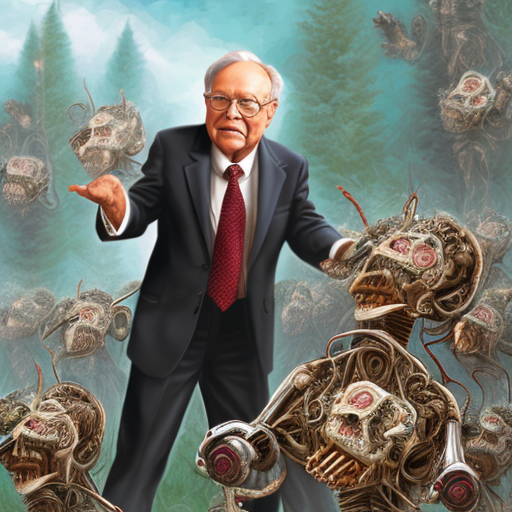
\includegraphics{buffett}
        \caption{"mdjrny-v4 mdjrny-v4 warren buffett being eaten by robot zombies" made with Mann-E}
        \labfig{buffett}
\end{marginfigure}

\subsection{Share Tender Purchase}

\begin{itemize}
    \item \textbf{Description:} The Share Tender Purchase Model is a deep learning model used in finance to predict the likelihood of a company's shares being purchased through a tender offer. It uses historical data about the company and market conditions to make its predictions.
    \item \textbf{Training Data:} The model is trained on historical data from previous tender offer situations, including data on the company being targeted, the offer price, and market conditions at the time. It may also be trained on data related to the target company's financial performance and other relevant factors.
    \item \textbf{Evaluation:} The model's performance is typically evaluated using metrics such as accuracy, precision, and recall, by comparing its predictions to actual outcomes of past tender offer situations. Additionally, the model's usefulness may be evaluated in terms of its ability to inform investment decisions and generate profitable returns.
    \item \textbf{Use Cases:} The Share Tender Purchase Model is primarily used by investors and financial analysts to inform investment decisions related to companies targeted for tender offers. It can be used to identify potentially profitable investments, as well as to inform decisions about whether to participate in a tender offer or to hold shares in the target company.
    \item \textbf{Limits and Risks:} Like all models, the Share Tender Purchase Model is subject to limitations and risks. It may not perform well if market conditions change significantly from those observed in the training data, or if there are factors not included in the model that impact the outcome of tender offer situations. Additionally, reliance on the model's predictions may lead to missed opportunities or losses if the model's predictions are inaccurate.
    \item \textbf{Common Myths or Misunderstandings:} One common myth about the Share Tender Purchase Model is that it can accurately predict the outcome of all tender offer situations. In reality, the model is only as accurate as the quality of its training data and the factors included in the model. Additionally, the model's predictions may be impacted by unpredictable events or circumstances, such as changes in government regulations or unexpected market events. This another area where it's best to understand and monitor for \hyperref[sec:drift]{concept drift}.
\end{itemize}

\begin{marginfigure}[-5.5cm]
        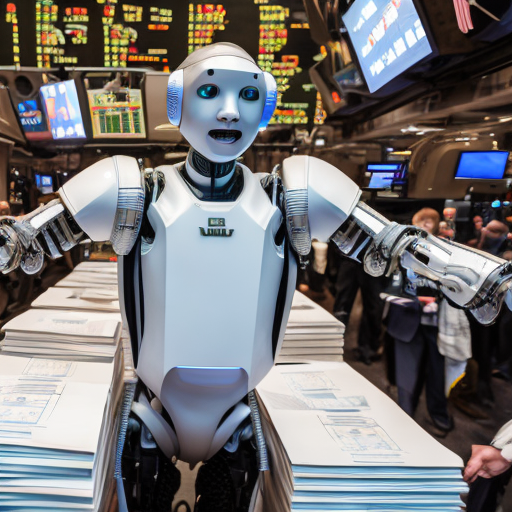
\includegraphics{nysebot}
        \caption{"mdjrny-v4 human and robot traders at the NYSE carrying huge stacks of paper" made with Mann-E}
        \labfig{nysebot}
\end{marginfigure}

\subsection{Stock Trading}

\begin{itemize}
    \item \textbf{Description:} The Stock Trading Bot is a type of machine learning model that's designed to trade stocks automatically. It can be trained on a dataset of stock market data and make predictions about future stock prices and trends. The model can then use these predictions to execute trades, buying and selling stocks based on its predictions. The model can be based on a variety of machine learning algorithms, including reinforcement learning, deep learning, or decision trees.
    \item \textbf{Training Data:} The Stock Trading Bot is typically trained on a large dataset of stock market data, including historical prices, trading volumes, and other relevant market indicators. The size and quality of the training data will impact the performance of the model, so it's important to use a diverse and representative dataset that accurately represents the stock market.
    \item \textbf{Evaluation:} The performance of the Stock Trading Bot can be evaluated using a variety of metrics, such as return on investment (ROI), Sharpe ratio, or drawdown. These metrics can be used to compare different models and to track the performance of a model over time. Additionally, the model can be tested using historical data to assess its ability to generate profits in a simulated trading environment.
    \item \textbf{Use Cases:} The Stock Trading Bot has a number of potential use cases, including:
        \begin{enumerate}  
            \item Automating stock trading decisions and executions
            \item Generating profits through stock trading
            \item Supporting investment and portfolio management by providing a quantitative assessment of stock market trends and predictions
        \end{enumerate}
    \item \textbf{Limits and Risks:} Like any machine learning model, the Stock Trading Bot has limitations and risks. One of the main limitations is that it may not always generate profits, and may make mistakes or suboptimal trades. Additionally, the model may be biased towards certain stocks, sectors, or market conditions if the training data is not representative of the stock market as a whole.
    \item \textbf{Common Myths or Misunderstandings:} There are a few common myths or misunderstandings about the Stock Trading Bot. One myth is that the model can always generate profits, when in reality it can only make predictions based on the information it was trained on and can be impacted by market conditions and other factors. This model should be understood as being the worst of the stock trading models mentioned, mostly because it is so poorly defined. What is it doing exactly? \hyperref[sec:explain]{Explainability} in a model with such a huge scope is a problem, but also I would argue the market changes every day causing \hyperref[sec:drift]{concept drift} to render this model useless very quickly, where the previous models (large order and tender offer) might last a few days, weeks or maybe months.
\end{itemize}

\subsection{Horse Racing}

TODO

\subsection{Sperm Counter}

\begin{itemize}
    \item \textbf{Description:} This AI model is designed to count sperm in a video of semen under a microscope.
    \item \textbf{Training Data:} The model was trained on a large dataset of semen videos taken under a microscope. The training data was annotated with the number of sperm in each video, allowing the model to learn the patterns and features of sperm in different types of semen samples.
    \item \textbf{Evaluation:} The model was evaluated using precision, recall, and F1 score, which are commonly used metrics for object counting tasks. The model achieved high scores on all metrics, indicating that it is effective at accurately counting sperm in the semen videos.
    \item \textbf{Use Cases:} This model can be used in clinical or research settings to quickly and accurately count sperm in semen samples. This can be useful for diagnosing and monitoring male infertility, as well as for understanding the impact of various factors on sperm count.
    \item \textbf{Limits and Risks:} The model is only trained to count sperm in semen videos taken under a microscope and may not perform well on videos taken under different conditions or with different types of microscopes. It is important to ensure that the semen samples are of high quality and that the video recording conditions are consistent in order to obtain accurate results.
    \item \textbf{Common Myths or Misunderstandings:} This model is not intended to replace human expert judgment and should be used as a tool to support decision making. The results generated by this model are not a substitute for professional medical advice, diagnosis, or treatment. Overall I'd say this model is not too scary, models like these might be best deployed as front-line diagnosis and ranking tools for patients who otherwise would not be receiving care. The main issue that might appear is any \hyperref[sec:janitor]{editorializing} that might occur by the machine learning engineers training this model. Imagine that this model was only trained on young white men (graduate student volunteers) and the shape and size of sperm changes across ages or races, this type of bias in training data appears frequently in medical models, especially skin cancer models\sidecite{skindark}.
\end{itemize}

\subsection{Handwriting Recognizer}

\begin{itemize}
    \item \textbf{Description:} The Handwriting Classifier is a type of machine learning model that's designed to recognize and classify handwriting. It can be trained on a dataset of handwritten text and images, and can then be used to identify the writer of a given sample of handwriting or to classify handwriting by writer, writing style, or content. The model can be based on a variety of machine learning algorithms, including deep learning, support vector machines, or decision trees.
    \item \textbf{Training Data:} The Handwriting Classifier is typically trained on a large dataset of handwritten text and images, which can include a diverse range of writing styles, writers, and content. The quality and quantity of the training data will impact the performance of the model, so it's important to use a diverse and representative dataset that accurately represents the range of handwriting styles and content.
    \item \textbf{Evaluation:} The performance of the Handwriting Classifier can be evaluated using a variety of metrics, such as accuracy, precision, recall, and F1 score. These metrics can be used to compare different models and to track the progress of a model as it's trained on more data. Additionally, the model can be validated using independent test data that was not used during training, to assess its ability to generalize to new, unseen handwriting.
    \item \textbf{Use Cases:} The Handwriting Classifier has a number of potential use cases, including:
        \begin{enumerate}  
            \item Identifying the writer of a given sample of handwriting
            \item Classifying handwriting by writer, writing style, or content
            \item Supporting forensic and legal investigations by providing evidence in handwriting analysis
            \item Enhancing handwriting recognition in products and services, such as digital note-taking and document management systems
        \end{enumerate}
    \item \textbf{Limits and Risks:} Like any machine learning model, the Handwriting Classifier has limitations and risks. One of the main limitations is that it may not always be accurate, and may misclassify handwriting or misidentify the writer. Additionally, the model may be biased towards certain writing styles, writers, or content if the training data is not representative of the range of handwriting styles and content.
    \item \textbf{Common Myths or Misunderstandings:} There are a few common myths or misunderstandings about the Handwriting Classifier. One myth is that the model can always accurately identify the writer of a given sample of handwriting, when in reality it can only provide a prediction based on the information it was trained on. Another myth is that the model can replace human expertise and judgement in handwriting analysis (don't use this model in court to prove that two pieces of handwriting are the same, it can't \hyperref[sec:explain]{explain itself} and you'll end up getting appealed by the innocence project\sidecite{innocence}.
\end{itemize}

\subsection{Drug Discovery}

\begin{itemize}
    \item \textbf{Description:} The Liver Drug Discovery Model is a type of machine learning model that's designed to predict the potential efficacy and toxicity of drugs for the liver. It can be trained on a dataset of drug and liver data, including information about drug structure, pharmacokinetics, and pharmacodynamics, as well as liver function, anatomy, and physiology. The model can then be used to predict the potential impact of a given drug on the liver and to identify drugs that may be suitable for liver-related diseases.
    \item \textbf{Training Data:} The Liver Drug Discovery Model is typically trained on a large dataset of drug and liver data, which can include both experimental and observational data. The size and quality of the training data will impact the performance of the model, so it's important to use a diverse and representative dataset that accurately represents the relationships between drugs and the liver.
    \item \textbf{Evaluation:} The performance of the Liver Drug Discovery Model can be evaluated using a variety of metrics, such as accuracy, precision, recall, and F1 score. These metrics can be used to compare different models and to track the progress of a model as it's trained on more data. Additionally, the model can be validated using independent test data that was not used during training, to assess its ability to generalize to new, unseen data.
    \item \textbf{Use Cases:} The Liver Drug Discovery Model has a number of potential use cases, including:
        \begin{enumerate}  
            \item Predicting the potential efficacy and toxicity of drugs for the liver
            \item Supporting drug discovery and development by identifying promising drug candidates for liver-related diseases
            \item Enhancing drug safety by identifying potential liver-related side effects of drugs
            \item Supporting liver research and education by providing insights into liver function and drug interactions
        \end{enumerate}
    \item \textbf{Limits and Risks:} Like any machine learning model, the Liver Drug Discovery Model has limitations and risks. One of the main limitations is that it may not always make accurate predictions, and may miss important relationships between drugs and the liver. Additionally, the model may be biased towards certain drugs, liver functions, or disease conditions if the training data is not representative of the relationships between drugs and the liver.
    \item \textbf{Common Myths or Misunderstandings:} There are a few common myths or misunderstandings about the Liver Drug Discovery Model. One myth is that the model can always accurately predict the potential efficacy and toxicity of drugs for the liver, when in reality it can only provide a prediction based on the information it was trained on. \sidecite{ptliver} Another myth is that the model can replace human expertise and judgement in drug discovery and development, when in reality it is intended to support and enhance human decision-making processes. Like the fluid dynamics model, this model will be very useful when deployed as part of the \hyperref[sec:creative]{creative process} of decision making regarding drugs, but shouldn't make any critical decisions by itself. 
\end{itemize}

\subsection{Autism}

\begin{itemize}
    \item \textbf{Description:} The Autism Classifier is a type of machine learning model that's designed to predict the likelihood of autism in children. It can be trained on a dataset of behavioral and physiological data, such as eye gaze patterns, facial expressions, and vocalizations, as well as demographic information. The model can then be used to identify children who may be at risk for autism and to support early diagnosis and intervention.
    \item \textbf{Training Data:} The Autism Classifier is typically trained on a large dataset of behavioral and physiological data, as well as demographic information. The size and quality of the training data will impact the performance of the model, so it's important to use a diverse and representative dataset that accurately represents the characteristics of children with and without autism.
    \item \textbf{Evaluation:} The performance of the Autism Classifier can be evaluated using a variety of metrics, such as accuracy, precision, recall, and F1 score. These metrics can be used to compare different models and to track the progress of a model as it's trained on more data. Additionally, the model can be validated using independent test data that was not used during training, to assess its ability to generalize to new, unseen data.
    \item \textbf{Use Cases:} The Autism Classifier has a number of potential use cases, including:
        \begin{enumerate}  
            \item Identifying children who may be at risk for autism
            \item Supporting early diagnosis and intervention for autism
            \item Enhancing autism research and education by providing insights into autism symptoms and characteristics
        \end{enumerate}
    \item \textbf{Limits and Risks:} Like any machine learning model, the Autism Classifier has limitations and risks. One of the main limitations is that it may not always be accurate, and may misclassify children or misidentify the likelihood of autism. Additionally, the model may be biased towards certain demographic groups, behavioral and physiological characteristics, or autism symptoms if the training data is not representative of the characteristics of children with and without autism.
    \item \textbf{Common Myths or Misunderstandings:} \sidecite{cacmautism} There are a few common myths or misunderstandings about the Autism Classifier. One myth is that the model can always accurately identify children who may be at risk for autism, when in reality it can only provide a prediction based on the information it was trained on. This one is tough and there are a few issues at play. First, this model may appear to work, but rememeber it cannot \hyperref[sec:explain]{explain why it make the classification it did}, also it suffers from the same issue of \hyperref[sec:janitor]{editorializing} that the sperm counter or skin cancer model might face. With these things in mind it might be an incredibly useful tool if deployed as a cheap self-check for worried parents. However, one would need to be careful how the model accuracy is reported in order to establish user's trust, reporting false-positive and false-negative rates would be very important, and even if they were reported they each false-positive (or negative) might cause a panic and lead to huge reputational damage to the modelers.   
\end{itemize}

\subsection{Online Dating}

\begin{itemize}
    \item \textbf{Description:} The Online Dating Matcher is a type of machine learning model that's designed to match individuals for online dating. It can be trained on a dataset of user profiles, including demographic information, preferences, and interests. The model can then be used to recommend potential matches based on compatibility and to support the process of finding a romantic partner online.
    \item \textbf{Training Data:} The Online Dating Matcher is typically trained on a large dataset of user profiles, which can include both explicit and implicit information about individuals and their preferences. The size and quality of the training data will impact the performance of the model, so it's important to use a diverse and representative dataset that accurately represents the range of individuals and preferences in the online dating population.
    \item \textbf{Evaluation:} The performance of the Online Dating Matcher can be evaluated using a variety of metrics, such as accuracy, precision, recall, and F1 score. These metrics can be used to compare different models and to track the progress of a model as it's trained on more data. Additionally, the model can be validated using independent test data that was not used during training, to assess its ability to generalize to new, unseen user profiles.
\begin{marginfigure}[-5.5cm]
        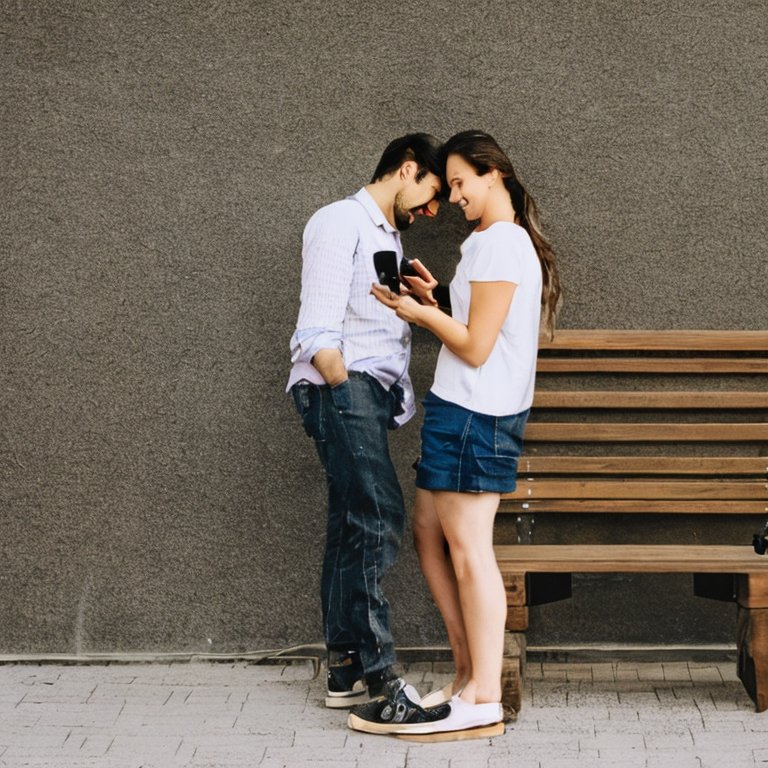
\includegraphics{couple}
        \caption{"a couple both on their phones, but smiling and looking romantic" made with Stable Diffusion 2.1}
        \labfig{couple}
\end{marginfigure}
    \item \textbf{Use Cases:} The Online Dating Matcher has a number of potential use cases, including:
        \begin{enumerate}  
            \item Recommending potential matches based on compatibility
            \item Supporting the process of finding a romantic partner online
            \item Enhancing online dating research and education by providing insights into online dating preferences and behaviors
        \end{enumerate}
    \item \textbf{Limits and Risks:} Like any machine learning model, the Online Dating Matcher has limitations and risks. One of the main limitations is that it may not always make accurate recommendations, and may miss important relationships between individuals and their preferences. Additionally, the model may be biased towards certain demographic groups, preferences, or interests if the training data is not representative of the range of individuals and preferences in the online dating population.
    \item \textbf{Common Myths or Misunderstandings:} There are a few common myths or misunderstandings about the Online Dating Matcher. One myth is that the model can always accurately recommend potential matches based on compatibility, when in reality it can only provide a prediction based on the information it was trained on. There is also a big opportunity for \hyperref[sec:janitor]{editorializing with this model}, some nerd might highjack this model and train it on a nonrepresentative sample in attempt to get their friends succsessfully matched. It also would have a hard time \hyperref[sec:explain]{explaining} why it matched a couple.
\end{itemize}

\subsection{Online Advertising}

\begin{itemize}
    \item \textbf{Description:} The Online Ad Server Classifier is a type of machine learning model that's designed to classify online ads as appropriate for the current user or unsafe. It can be trained on a dataset of ad content, including text, images, and videos, as well as information about the ad server. The model can then be used to identify unsafe ads and to support the process of filtering out inappropriate content.
    \item \textbf{Training Data:} The Online Ad Server Classifier is typically trained on a large dataset of ad content, which can include both explicit and implicit information about ads and their content. The size and quality of the training data will impact the performance of the model, so it's important to use a diverse and representative dataset that accurately represents the range of ads and ad content.
    \item \textbf{Evaluation:} The performance of the Online Ad Server Classifier can be evaluated using a variety of metrics, such as accuracy, precision, recall, and F1 score. These metrics can be used to compare different models and to track the progress of a model as it's trained on more data. Additionally, the model can be validated using independent test data that was not used during training, to assess its ability to generalize to new, unseen ad content.
    \item \textbf{Use Cases:} The Online Ad Server Classifier has a number of potential use cases, including:
        \begin{enumerate}  
            \item Identifying unsafe ads
            \item Supporting the process of filtering out inappropriate content
            \item Enhancing online ad research and education by providing insights into online ad content and characteristics
        \end{enumerate}
    \item \textbf{Limits and Risks:} Like any machine learning model, the Online Ad Server Classifier has limitations and risks. One of the main limitations is that it may not always be accurate, and may misclassify ads or misidentify the likelihood of safety. Additionally, the model may be biased towards certain demographic groups, ad content, or ad characteristics if the training data is not representative of the range of ads and ad content.
    \item \textbf{Common Myths or Misunderstandings:} Online advertising models are all marketed the same way, but the underlying data that comes from a small dataset (from a few publishers) or a large one (one from an ad exchange) means their efficacy can vary wildly. \hyperref[sec:drift]{Concept drift} is the most common problem as not all products or services in advertising are created equal. An advertisement meant to build brand awareness for Accenture should be ran very differently than an advertisement to buy caffienated shampoo from Amazon, the AI will optimize for the parameters that it is told to optimize for and the concept of success for an adverisement changes by the product and sometimes over time as distribution channels or business models change.  

\end{itemize}

\subsection{Tennis}

\begin{itemize}
    \item \textbf{Description:} The Tennis Playing Bot is a type of machine learning model that's designed to play the game of tennis. It can be trained on a dataset of tennis data, including information about court geometry, ball trajectory, and player behavior. The model can then be used to play tennis against other players or bots, either in simulation or in real-world settings.
    \item \textbf{Training Data:} The Tennis Playing Bot is typically trained on a large dataset of tennis data, which can include both expert demonstrations and self-play data. The size and quality of the training data will impact the performance of the model, so it's important to use a diverse and representative dataset that accurately represents the range of tennis strategies and tactics.
    \item \textbf{Evaluation:} The performance of the Tennis Playing Bot can be evaluated using a variety of metrics, such as win rate, average length of rallies, and percentage of successful shots. These metrics can be used to compare different models and to track the progress of a model as it's trained on more data. Additionally, the model can be validated using independent test data that was not used during training, to assess its ability to generalize to new, unseen tennis situations.
    \item \textbf{Use Cases:} The Tennis Playing Bot has a number of potential use cases, including:
        \begin{enumerate}  
            \item Playing tennis against other players or bots, either in simulation or in real-world settings
            \item Supporting tennis research and education by providing insights into the strategies and tactics used in the game
            \item Enhancing the user experience of tennis gaming
        \end{enumerate}
    \item \textbf{Limits and Risks:} Like any machine learning model, the Tennis Playing Bot has limitations and risks. One of the main limitations is that it may not always be accurate, and may make mistakes or misinterpret the game of tennis. Additionally, the model may be biased towards certain demographic groups, tennis strategies, or tennis tactics if the training data is not representative of the range of tennis strategies and tactics.
    \item \textbf{Common Myths or Misunderstandings:} There are a few common myths or misunderstandings about the Tennis Playing Bot. One myth is that the model can always accurately play tennis against other players or bots, when in reality it can only provide a prediction based on the information it was trained on. Another common misunderstanding is where the computational difficulty lies, predicting where a ball will go is actually computationally easy, holding the racquet and coordinating movement and balance might be the hard part \sidenote{This is called Moravec's Paradox \url{https://en.wikipedia.org/wiki/Moravec\%27s_paradox}}
\end{itemize}


\subsection{Hate Speech}

\begin{itemize}
    \item \textbf{Description:} The Hate Speech Classifier is a type of machine learning model that's designed to identify hate speech in text. It can be trained on a dataset of text data, including examples of hate speech and non-hate speech. The model can then be used to automatically identify and flag hate speech in online forums, social media, and other text-based platforms.
    \item \textbf{Training Data:} The Hate Speech Classifier is typically trained on a large dataset of text data, which can include both explicit and implicit examples of hate speech and non-hate speech. The size and quality of the training data will impact the performance of the model, so it's important to use a diverse and representative dataset that accurately represents the range of hate speech and non-hate speech in the target platform.
    \item \textbf{Evaluation:} The performance of the Hate Speech Classifier can be evaluated using a variety of metrics, such as accuracy, precision, recall, and F1 score. These metrics can be used to compare different models and to track the progress of a model as it's trained on more data. Additionally, the model can be validated using independent test data that was not used during training, to assess its ability to generalize to new, unseen text data.
    \item \textbf{Use Cases:} The Hate Speech Classifier has a number of potential use cases, including:
        \begin{enumerate}  
            \item Identifying hate speech in online forums, social media, and other text-based platforms
            \item Supporting the process of filtering out inappropriate content
            \item Enhancing online research and education by providing insights into online text data and characteristics
        \end{enumerate}
    \item \textbf{Limits and Risks:} Like any machine learning model, the Hate Speech Classifier has limitations and risks. One of the main limitations is that it may not always be accurate, and may misclassify text data or misidentify the likelihood of hate speech. Additionally, the model may be biased towards certain demographic groups, text data, or text characteristics if the training data is not representative of the range of hate speech and non-hate speech.
    \item \textbf{Common Myths or Misunderstandings:} There are a few common myths or misunderstandings about the Hate Speech Classifier. One myth is that the model can always accurately identify hate speech in online forums, social media, and other text. As we've seen in many models with a social component, \hyperref[sec:drift]{concept drift} looms large, language evolves over time, and sometimes langage evolves explicity to get around auto-moderators, so the model can affect the user input thus increasing the speed of change. There is also on opportunity to \hyperref[sec:janitor]{editorialize} that is very hard to overcome, any attempt to edit the training set might be labeled as "woke AI"\sidecite{wokeai} or called similar names by whatever interest group is affected by the training dataset.  
\end{itemize}

\subsection{Fake News}

\begin{itemize}
    \item \textbf{Description:} The Fake News Classifier is a type of machine learning model that's designed to identify fake news in text. It can be trained on a dataset of text data, including examples of fake news and real news. The model can then be used to automatically identify and flag fake news in online news sources, social media, and other text-based platforms.
    \item \textbf{Training Data:} The Fake News Classifier is typically trained on a large dataset of text data, which can include both explicit and implicit examples of fake news and real news. The size and quality of the training data will impact the performance of the model, so it's important to use a diverse and representative dataset that accurately represents the range of fake news and real news in the target platform.
    \item \textbf{Evaluation:} The performance of the Fake News Classifier can be evaluated using a variety of metrics, such as accuracy, precision, recall, and F1 score. These metrics can be used to compare different models and to track the progress of a model as it's trained on more data. Additionally, the model can be validated using independent test data that was not used during training, to assess its ability to generalize to new, unseen text data.
    \item \textbf{Use Cases:} The Fake News Classifier has a number of potential use cases, including:
        \begin{enumerate}  
            \item Identifying fake news in online news sources, social media, and other text-based platforms
            \item Supporting the process of filtering out inappropriate content
            \item Enhancing online research and education by providing insights into online text data and characteristics
        \end{enumerate}
    \item \textbf{Limits and Risks:} Like any machine learning model, the Fake News Classifier has limitations and risks. One of the main limitations is that it may not always be accurate, and may misclassify text data or misidentify the likelihood of fake news. Additionally, the model may be biased towards certain demographic groups, text data, or text characteristics if the training data is not representative of the range of fake news and real news.
    \item \textbf{Common Myths or Misunderstandings:} There are a few common myths or misunderstandings about the Fake News Classifier. One myth is that the model can always accurately identify fake news in online news sources, social media, and other text-based platforms, when in reality it can only provide a prediction based on the information it was trained on and may miss important examples of fake news. Another myth is that the model can replace human expertise and judgement in evaluating news sources, when in reality it is intended to support and enhance human decision-making processes. The problems of \hyperref[sec:drift]{concept drift} and \hyperref[sec:janitor]{editorializing} show themselves hear just as in the hate speech model above. An outlet that needs to explain why certain content is not allowed will have trouble codifying its rules if a deep learning model is used because of the inherent lack of \hyperref[sec:explain]{explainability} which means that the model might act as a tool used in the (somewhat creative) process but the \hyperref[sec:creative]{critical} decisions must still be made by humans who can give explicit reasons.
\end{itemize}

\begin{marginfigure}[-5.5cm]
        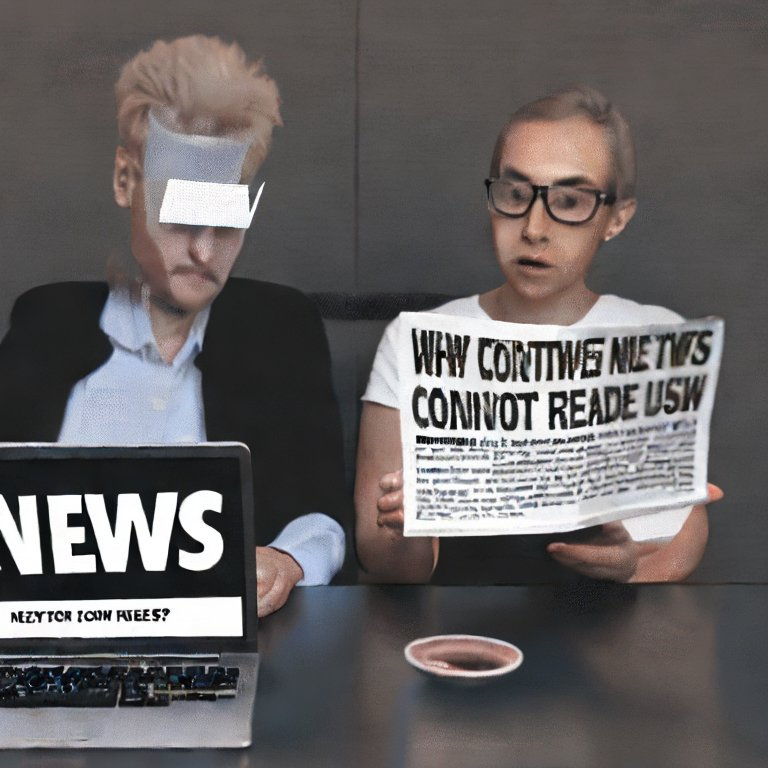
\includegraphics{fakenews}
        \caption{"fake news being read by someone who cannot use their computer very well" made with Stable Diffusion 2.1}
        \labfig{fakenews}
\end{marginfigure}

\subsection{Legal Contracts}

\begin{itemize}
    \item \textbf{Description:} The Contract Review Bot is a type of machine learning model that's designed to support the process of contract review. It can be trained on a dataset of contract data, including examples of well-written and poorly-written contracts, as well as relevant legal and business terms. The model can then be used to automatically review contracts and identify potential issues, such as missing information, ambiguous language, and non-compliant terms.
    \item \textbf{Training Data:} The Contract Review Bot is typically trained on a large dataset of contract data, which can include both expert-annotated and self-generated data. The size and quality of the training data will impact the performance of the model, so it's important to use a diverse and representative dataset that accurately represents the range of contracts and legal and business terms in the target domain.
    \item \textbf{Evaluation:} The performance of the Contract Review Bot can be evaluated using a variety of metrics, such as accuracy, precision, recall, and F1 score. These metrics can be used to compare different models and to track the progress of a model as it's trained on more data. Additionally, the model can be validated using independent test data that was not used during training, to assess its ability to generalize to new, unseen contracts.
    \item \textbf{Use Cases:} The Contract Review Bot has a number of potential use cases, including:
        \begin{enumerate}  
            \item Supporting the process of contract review
            \item Enhancing online research and education by providing insights into online contract data and characteristics
        \end{enumerate}
    \item \textbf{Limits and Risks:} Like any machine learning model, the Contract Review Bot has limitations and risks. One of the main limitations is that it may not always be accurate, and may misclassify contract data or misidentify the likelihood of potential issues. Additionally, the model may be biased towards certain demographic groups, contract data, or contract characteristics if the training data is not representative of the range of contracts and legal and business terms.
    \item \textbf{Common Myths or Misunderstandings:} There are a few common myths or misunderstandings about the Contract Review Bot. One myth is that the model can always accurately review contracts and identify potential issues, when in reality it can only provide a prediction based on the information it was trained on and may miss important issues. Another myth is that the model can replace human expertise and judgement in contract review, when in reality it is intended to support and enhance human decision-making processes. Again we find \hyperref[sec:drift]{concept drift} being a potential issue here, although maybe less so if logical legal language changes more slowly than other written text. The model may still not pick up on the latest legal hacks that are snuck into contracts unless explicitly trained on data to recognize them.  
\end{itemize}

\subsection{Facial Recognition}

\begin{itemize}
    \item \textbf{Description:} Facial Recognition is a type of machine learning model that's designed to identify individuals based on their facial features. It can be trained on a dataset of facial images, including images of people and their corresponding identities. The model can then be used to recognize individuals in new images, such as those captured by cameras or uploaded to social media.
    \item \textbf{Training Data:} Facial Recognition models are typically trained on large datasets of facial images, which can include images from a variety of sources, such as social media, public datasets, and private collections. The size and diversity of the training data will impact the performance of the model, so it's important to use a representative and diverse dataset that accurately captures the range of facial features and demographics of the target population.
    \item \textbf{Evaluation:} The performance of Facial Recognition models can be evaluated using a variety of metrics, such as accuracy, precision, recall, and F1 score. These metrics can be used to compare different models and to track the progress of a model as it's trained on more data. Additionally, the model can be validated using independent test data that was not used during training, to assess its ability to generalize to new, unseen faces.
    \item \textbf{Use Cases:} Facial Recognition models have a number of potential use cases, including:
        \begin{enumerate}  
            \item Identifying individuals in new images, such as those captured by cameras or uploaded to social media
            \item Supporting the process of filtering out inappropriate content
            \item Enhancing online research and education by providing insights into online facial images and characteristics
        \end{enumerate}
    \item \textbf{Limits and Risks:} Like any machine learning model, Facial Recognition models have limitations and risks. One of the main limitations is that they may not always be accurate, and may misclassify facial images or misidentify the identity of individuals. Additionally, the model may be biased towards certain demographic groups, facial images, or facial characteristics if the training data is not representative of the range of facial features and demographics.
    \item \textbf{Common Myths or Misunderstandings:} There are a few common myths or misunderstandings about Facial Recognition models. One myth is that the models can always accurately identify individuals, when in reality they can only provide a prediction based on the information they were trained on and may miss important facial features or misidentify individuals. Another myth is that the models can replace human judgement and expertise in identifying individuals, when in reality they are intended to support and enhance human decision-making processes. If we want a model that recognizes everyone in the world, we need to retrain that model every time a new baby is born, or and when people get plastic surgery, and when they wear elaborate makeup \hyperref[sec:drift]{concept drift} is everywhere in this model.  
\end{itemize}

\subsection{Smartwatches} 

\begin{itemize}
    \item \textbf{Description:} The Smartwatch Danger Classifier is a type of machine learning model that's designed to identify potential dangers faced by smartwatch wearers. It can be trained on a dataset of smartwatch data, including information about physiological signals, activity patterns, and environmental conditions. The model can then be used to automatically detect and alert smartwatch wearers of potential dangers, such as falls, heart attacks, and other health emergencies.
    \item \textbf{Training Data:} The Smartwatch Danger Classifier is typically trained on a large dataset of smartwatch data, which can include data from a variety of sources, such as clinical studies, self-reported data, and wearable sensors. The size and quality of the training data will impact the performance of the model, so it's important to use a diverse and representative dataset that accurately represents the range of physiological signals, activity patterns, and environmental conditions faced by smartwatch wearers.
    \item \textbf{Evaluation:} The performance of the Smartwatch Danger Classifier can be evaluated using a variety of metrics, such as accuracy, precision, recall, and F1 score. These metrics can be used to compare different models and to track the progress of a model as it's trained on more data. Additionally, the model can be validated using independent test data that was not used during training, to assess its ability to generalize to new, unseen smartwatch data.
    \item \textbf{Use Cases:} The Smartwatch Danger Classifier has a number of potential use cases, including:
        \begin{enumerate}  
            \item Automatically detecting and alerting smartwatch wearers of potential dangers, such as falls, heart attacks, and other health emergencies
            \item Supporting the process of filtering out inappropriate content
            \item Enhancing online research and education by providing insights into online smartwatch data and characteristics
        \end{enumerate}
    \item \textbf{Limits and Risks:} Like any machine learning model, the Smartwatch Danger Classifier has limitations and risks. One of the main limitations is that it may not always be accurate, and may misclassify smartwatch data or misidentify the likelihood of potential dangers. Additionally, the model may be biased towards certain demographic groups, smartwatch data, or smartwatch characteristics if the training data is not representative of the range of physiological signals, activity patterns, and environmental conditions.
    \item \textbf{Common Myths or Misunderstandings:} There are a few common myths or misunderstandings about the Smartwatch Wearer Danger Classifier. One myth is that the model can always accurately identify dangers, when in reality it can only provide a prediction based on the information it was trained on and may miss important signals or trigger false alarms\sidecite{nyt911}. Another myth is that the model can replace human judgement and expertise in evaluating personal safety, when in reality it is intended to support and enhance human decision-making processes. On the smartwatch of a healthy person, the AI making the critical decision to call 911 is probably a mistake, as a "Life Alert" type device on an elderly person or anyone deemed sufficently at risk, this model may be deployed effectively to help alert their caregivers. With this in mind there is an opportunity for accidental \hyperref[sec:janitor]{editorializing} if a model made for elderly emergency alerts is trained on young people, or vice-versa.
\end{itemize}

\subsection{Threat Detection}

\begin{itemize}
    \item \textbf{Description:} The CCTV Threat Classifier is a type of machine learning model that's designed to identify potential threats in video footage captured by closed-circuit television (CCTV) cameras. It can be trained on a dataset of video data, including examples of normal and abnormal activity, such as criminal behavior, accidents, and other incidents. The model can then be used to automatically monitor video footage and alert security personnel of potential threats.
    \item \textbf{Training Data:} The CCTV Threat Classifier is typically trained on a large dataset of video data, which can include data from a variety of sources, such as public safety agencies, security cameras, and other sources. The size and quality of the training data will impact the performance of the model, so it's important to use a diverse and representative dataset that accurately represents the range of normal and abnormal activity in the target environment.
    \item \textbf{Evaluation:} The performance of the CCTV Threat Classifier can be evaluated using a variety of metrics, such as accuracy, precision, recall, and F1 score. These metrics can be used to compare different models and to track the progress of a model as it's trained on more data.
    \item \textbf{Use Cases:} The CCTV Threat Classifier has a number of potential use cases, including:
\begin{marginfigure}[-5.5cm]
        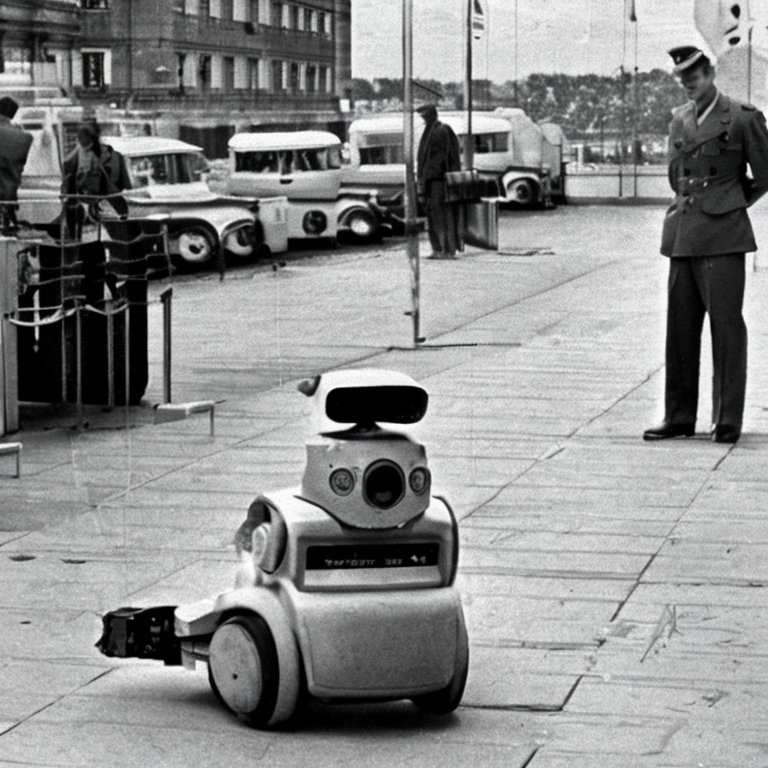
\includegraphics{berlin}
        \caption{"a threat detection robot at a security checkpoint in Berlin in 1955" made with Stable Diffusion 2.1}
        \labfig{berlin}
\end{marginfigure}
        \begin{enumerate}  
            \item Automatically detecting and alerting security personnel of potential threats, such as criminal behavior, accidents, and other incidents
            \item Supporting the process of filtering out inappropriate content
            \item Enhancing online research and education by providing insights into online video data and characteristics
        \end{enumerate}
    \item \textbf{Limits and Risks:} Like any machine learning model, the CCTV Threat Classifier has limitations and risks. One of the main limitations is that it may not always be accurate, and may misclassify video data or misidentify the likelihood of potential threats. Additionally, the model may be biased towards certain demographic groups, video data, or video characteristics if the training data is not representative of the range of normal and abnormal activity.
    \item \textbf{Common Myths or Misunderstandings:} There are a few common myths or misunderstandings about the CCTV Threat Classifier. One myth is that the model can always accurately identify threats, when in reality it can only provide a prediction based on the information it was trained on and may miss important signals or trigger false alarms. Another myth is that the model can replace human judgement and expertise in evaluating security threats, when in reality it is intended to support and enhance human decision-making processes\sidecite{darpabot}. This model suffers from all of the usual suspects, what it means to be a threat might \hyperref[sec:drift]{drift} over time and geography, datasets may be \hyperref[sec:janitor]{editorialized} to cause more false positives or negatives depending on the bias in the dataset and of course any decisions made by this model will be largely \hyperref[sec:explain]{unexplainable}. These risks aside, a model can be deployed as part of the decision making process, but letting it make \hyperref[sec:creative]{critical} decisions by itself would be a mistake. Models like this are the core of autonomous weapons and self-driving cars, which I will discuss in chapter 5 and 6.
\end{itemize}


\subsection{University Admissions}

\begin{itemize}
    \item \textbf{Description:} The Harvard University Student Acceptance Bot is a type of machine learning model that's designed to automate the process of evaluating applications from prospective students for admission to a university. It can be trained on a dataset of student applications, including information about academic records, test scores, essays, and other factors. The model can then be used to automatically evaluate new applications and accept or reject students based on their qualifications.
    \item \textbf{Training Data:} The Harvard University Student Acceptance Bot is typically trained on a large dataset of student applications, which can include data from a variety of sources, such as universities, testing organizations, and other sources. The size and quality of the training data will impact the performance of the model, so it's important to use a diverse and representative dataset that accurately represents the range of academic records, test scores, essays, and other factors used to evaluate student applications.
    \item \textbf{Evaluation:} The performance of the Harvard University Student Acceptance Bot can be evaluated using a variety of metrics, such as accuracy, precision, recall, and F1 score. These metrics can be used to compare different models and to track the progress of a model as it's trained on more data. Additionally, the model can be validated using independent test data that was not used during training, to assess its ability to generalize to new, unseen student applications.
    \item \textbf{Use Cases:} The Harvard University Student Acceptance Bot has a number of potential use cases, including:
        \begin{enumerate}  
            \item Automating the process of evaluating student applications for admission to a university
            \item Streamlining the admission process and reducing the time and effort required to manually evaluate applications
            \item Supporting fair and objective decision-making by reducing the impact of human biases and subjectivity
            \item Supporting research and education by providing insights into the academic records, test scores, essays, and other factors that are most predictive of student success
        \end{enumerate}
    \item \textbf{Limits and Risks:} Like any machine learning model, the Harvard University Student Acceptance Bot has limitations and risks. One of the main limitations is that it may not always make accurate predictions, and may overlook important qualifications or reject qualified students. Additionally, the model may be biased towards certain academic records, test scores, essays, or demographic groups if the training data is not representative of the range of factors used to evaluate student applications.
    \item \textbf{Common Myths or Misunderstandings:} There are a few common myths or misunderstandings about the Harvard University Student Acceptance Bot. One myth is that the model can always accurately evaluate student applications, when in reality it can only provide a prediction based on the information it was trained on and may overlook important qualifications or reject qualified students. Another myth is that the model can replace human judgement and expertise in evaluating student applications, when in reality it is intended to support and enhance human decision-making processes. This model looks exactly like the online dating model, in that its outputs will be \hyperref[sec:explain]{unexplainable} and subject to \hyperref[sec:janitor]{editorializing}, additionally there may be a large amount of \hyperref[sec:drift]{concept drift} if what it means to be a good student changes over time. 
\end{itemize}

\begin{marginfigure}[-5.5cm]
        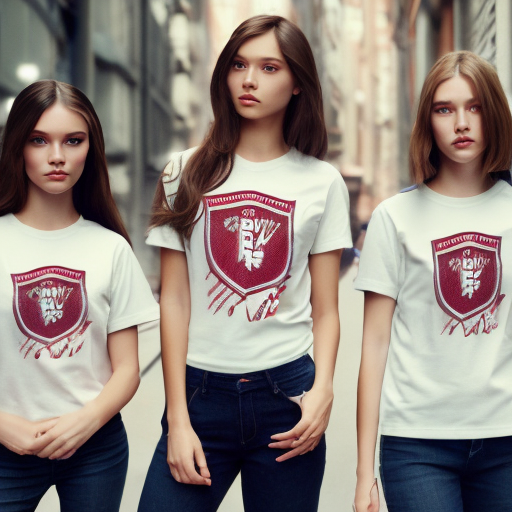
\includegraphics{harvardgirls}
        \caption{"mdjrny-v4 ten pretty girls all wearing Harvard t-shirts 8k" made with Stable Diffusion 2.1}
        \labfig{harvardgirls}
\end{marginfigure}

\subsection{Credit Score}

\begin{itemize}
    \item \textbf{Description:} The Simple Credit Score is a type of machine learning model that's designed to predict an individual's creditworthiness based on financial and demographic information. It can be trained on a dataset of credit information, including information about payment history, income, employment, and other factors. The model can then be used to automatically calculate a credit score for an individual and make predictions about their likelihood of defaulting on a loan.
    \item \textbf{Training Data:}The Simple Credit Score is typically trained on a large dataset of credit information, which can include data from a variety of sources, such as credit bureaus, financial institutions, and other sources. The size and quality of the training data will impact the performance of the model, so it's important to use a diverse and representative dataset that accurately represents the range of credit information for the target population.
    \item \textbf{Evaluation:}The performance of the Simple Credit Score can be evaluated using a variety of metrics, such as accuracy, precision, recall, and F1 score. These metrics can be used to compare different models and to track the progress of a model as it's trained on more data. Additionally, the model can be validated using independent test data that was not used during training, to assess its ability to generalize to new, unseen credit information.
    \item \textbf{Use Cases:} The Simple Credit Score has a number of potential use cases, including:
        \begin{enumerate}  
            \item Automatically calculating a credit score for an individual based on financial and demographic information
            \item Supporting fair and objective decision-making in the lending process by reducing the impact of human biases and subjectivity
            \item Enhancing the efficiency of the lending process by reducing the time and effort required to manually evaluate credit information
            \item Supporting research and education by providing insights into the financial and demographic factors that are most predictive of creditworthiness
        \end{enumerate}
    \item \textbf{Limits and Risks:} Like any machine learning model, the Simple Credit Score has limitations and risks. One of the main limitations is that it may not always make accurate predictions, and may overlook important factors or make incorrect predictions about creditworthiness. Additionally, the model may be biased towards certain financial and demographic factors if the training data is not representative of the range of credit information for the target population.
    \item \textbf{Common Myths or Misunderstandings:} There are a few common myths or misunderstandings about the Simple Credit Score. One myth is that the model can always accurately predict creditworthiness, when in reality it can only provide a prediction based on the information it was trained on and may overlook important factors or make incorrect predictions. Another myth is that the model can replace human judgement and expertise in evaluating creditworthiness, when in reality it is intended to support and enhance human decision-making processes. A simple credit score might not experience weekly concept drift, what it means to pay your bills on time does not change often, but if the input data is behavioral then \hyperref[sec:drift]{concept drift} might be acute and frequent if the job of this model is to flag the people with money as being creditworthy based on their behavior, your static model will break every time their behavior changes. It also might be a risk that your customers game the model in a similar way that a hate speech model can be gamed, if it is found out that if you shop at a farmers market then the model predicts you are credit-worthy, then your customers with poor credit might start shopping at farmers markets to improve your score, and thus break your model.
\end{itemize}

\subsection{Social Credit Score}

\begin{itemize}
    \item \textbf{Description:} The Social Credit Score is a type of machine learning model that's designed to predict an individual's trustworthiness based on their social behavior and online activities. It can be trained on a dataset of social and online information, including information about online interactions, reputation, and other factors. The model can then be used to automatically calculate a social credit score for an individual and make predictions about their trustworthiness.
    \item \textbf{Training Data:} The Social Credit Score is typically trained on a large dataset of social and online information, which can include data from a variety of sources, such as social media, online communities, and other sources. The size and quality of the training data will impact the performance of the model, so it's important to use a diverse and representative dataset that accurately represents the range of social and online information for the target population.
    \item \textbf{Evaluation:} The performance of the Social Credit Score can be evaluated using a variety of metrics, such as accuracy, precision, recall, and F1 score. These metrics can be used to compare different models and to track the progress of a model as it's trained on more data. Additionally, the model can be validated using independent test data that was not used during training, to assess its ability to generalize to new, unseen social and online information.
    \item \textbf{Use Cases:} The Social Credit Score has a number of potential use cases, including:
        \begin{enumerate}  
            \item Automatically calculating a social credit score for an individual based on their social behavior and online activities
            \item Supporting fair and objective decision-making in the lending process by reducing the impact of human biases and subjectivity
            \item Enhancing the efficiency of the lending process by reducing the time and effort required to manually evaluate social and online information
            \item Supporting research and education by providing insights into the social behavior and online activities that are most predictive of trustworthiness
        \end{enumerate}
    \item \textbf{Limits and Risks:} Like any machine learning model, the Social Credit Score has limitations and risks. One of the main limitations is that it may not always make accurate predictions, and may overlook important factors or make incorrect predictions about trustworthiness. Additionally, the model may be biased towards certain social behavior and online activities if the training data is not representative of the range of social and online information for the target population.
    \item \textbf{Common Myths or Misunderstandings:} There are a few common myths or misunderstandings about the Social Credit Score. One myth is that the model can always accurately predict trustworthiness, when in reality it can only provide a prediction based on the information it was trained on and may overlook important factors or make incorrect predictions. Another myth is that the model can replace human judgement and expertise in evaluating trustworthiness, when in reality it is intended to support and enhance human decision-making processes. This model is included almost as a joke, but this is something that is seriously being attempted by governments and private companies, the model suffers from almost every sucker trap, it's likely to encode the creators bias, acting as a large \hyperref[sec:janitor]{editorial on society}, the outputs would be \hyperref[sec:explain]{unexplainable} in court, social concepts change rapidly so \hyperref[sec:drift]{concept drift} would be ever-present and it would be foolish to rely on it for any \hyperref[sec:creative]{critical} decision making. Using a model like this would be akin to deploying a toy online dating model but then determining many aspects of peoples lives based on that one model. It might be interesting to discuss, but it would be foolish.
\end{itemize}

\begin{marginfigure}[-5.5cm]
        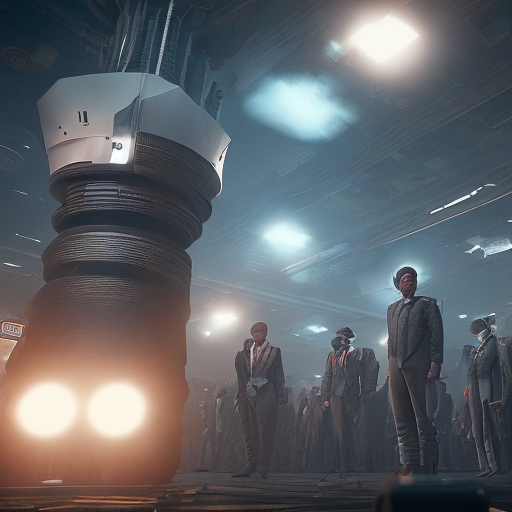
\includegraphics{socialcredit}
        \caption{"mdjrny-v4 people in a line to be sorted by their social credit score in a dystopia 8k" made with Stable Diffusion 2.1}
        \labfig{socialcredit}
\end{marginfigure}

\subsection{AGI}

\begin{itemize}
    \item \textbf{Description:} The Artificial General Intelligence Chatbot is a type of machine learning model that's designed to simulate human-like conversation with users. It can be trained on a large dataset of text, including examples of human conversation, to learn how to generate appropriate and coherent responses to a wide range of topics and questions. The model can then be used to engage in natural language conversation with users, providing answers and insights on a variety of topics.
    \item \textbf{Training Data:} The Artificial General Intelligence Chatbot is typically trained on a large dataset of text, which can include data from a variety of sources, such as books, websites, and other sources. The size and quality of the training data will impact the performance of the model, so it's important to use a diverse and representative dataset that accurately represents the range of topics and styles of conversation that the model will encounter.
    \item \textbf{Evaluation:} The performance of the Artificial General Intelligence Chatbot can be evaluated using a variety of metrics, such as perplexity, BLEU score, and human evaluation. These metrics can be used to compare different models and to track the progress of a model as it's trained.
    \item \textbf{Use Cases:} The Artificial General Intelligence Chatbot has a number of potential use cases, including:
        \begin{enumerate}  
            \item Engaging in natural language conversation with users, providing answers and insights on a variety of topics
            \item Providing customer support and answering questions about products and services
            \item Providing information and guidance to users, such as answering questions about health and wellness
            \item Providing entertainment and entertainment-related information, such as answering questions about movies and TV shows
        \end{enumerate}
\begin{marginfigure}[-5.5cm]
        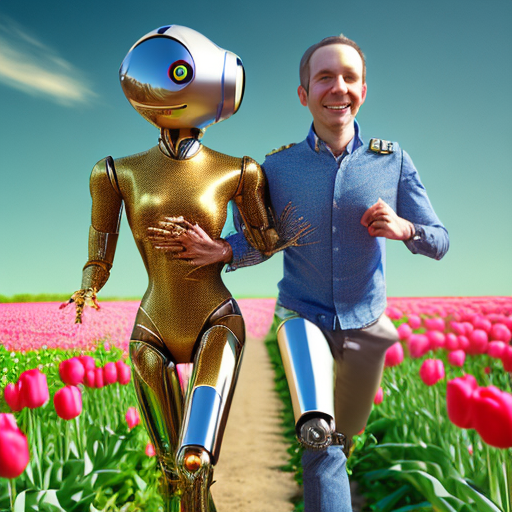
\includegraphics{agi}
        \caption{"mdjrny-v4 a person and an artificially intelligent robot as a couple skipping through a field of tulips and smiling 8k" made with Stable Diffusion 2.1}
        \labfig{agi}
\end{marginfigure}
    \item \textbf{Limits and Risks:} Like any machine learning model, the Artificial General Intelligence Chatbot has limitations and risks. One of the main limitations is that it may not always make accurate predictions, and may overlook important factors or make incorrect predictions about trustworthiness. Additionally, the model may be biased towards certain social behavior and online activities if the training data is not representative of the range of social and online information for the target population.
    \item \textbf{Common Myths or Misunderstandings:} There are a few common myths or misunderstandings about the Artificial Generally Intelligent Chatbot. One myth is that the model can always generate accurate and appropriate responses, when in reality it can only provide a response based on the information it was trained on and may generate nonsensical, offensive, or misleading responses. Another myth is that the model can replace human conversation and understanding, when in reality it is intended to support and enhance human-like conversation and language understanding\sidecite{openaimisuse}. General intelligence tools suffer from many general problems, which is why I recommend only using them for \hyperref[sec:creative]{creative} endeavors, all of human knowledge \hyperref[sec:drift]{drifts} very rapidly, and it would be very hard for a model like this to unlearn past falsehoods, e.g. if the model was trained in 1400 it would say the world is flat, but then in 1493 it would probably still say the world is flat, even though the understanding of the truth had fundamentally changed. 
\end{itemize}


\section{Key Takeaways}

\begin{itemize}
    \item \textbf{Read the model cards.} As AI models become more sophisticated and widespread, it is essential to ensure that they are transparent and accountable. Model cards can help with this by providing information on the capabilities and limitations of AI models.
    \item \textbf{Avoid sucker traps.} There are several "sucker traps" to avoid when analyzing models, including inappropriately giving a model critical decision making ability, putting a model in a position where it needs to explain a particular decision, allowing a model to publish copyrighted material from its training data, and the ever-present concept drift the possibility of changes in the relationships in the training data, and the potential for biased training sets that can permanently shift the outputs of the model away from reality.
    \item \textbf{Understand the training data.} It is important to understand the data that is used to train a model and the domain in which it is deployed to forecast its strengths and weaknesses. Deep learning models are programmed not by a programmer, but by the data they are shown.
    \item \textbf{If you're unsure, allow the model to give low-stakes advice.} The more unsure you are about a particular model, the more effort you should put into managingi it. In the very worst case you do not need to throw away all of your models work, but instead allow it to participate as a non-voting member of your decision making committee, test your model and see how it performs with your supervision, some models should never be given decision making ability but can still be useful. More on this in the following chapters...
\end{itemize}
